%
% Projekt:		DOKU: IFJ, IAL
% Autor:		Radek Pistelak, xpiste04@stud.fit.vutbr.cz 
%

\documentclass[a4paper, 11pt, titlepage]{article}
\usepackage[left=2cm,text={17cm,24cm},top=3cm]{geometry}
\usepackage[czech]{babel}
\usepackage[utf8]{inputenc}
\usepackage[IL2]{fontenc}

\usepackage{algorithmic}
\usepackage{graphicx}
\usepackage{hyperref}
\usepackage{wrapfig}

\usepackage{natbib}             % sazba pouzite literatury
\usepackage{url}                % sazba URL

\usepackage{url}

\usepackage{listings}

\begin{document}

%%%%%%%%%%%%%%%%%%%%%%%%%%%%%%%%%%%%%%%%%%%%%%%%%%%%%%%%%%%%%%%%%%%%%%%%%
% ------ Titulní strana
%%%%%%%%%%%%%%%%%%%%%%%%%%%%%%%%%%%%%%%%%%%%%%%%%%%%%%%%%%%%%%%%%%%%%%%%%
\begin{titlepage}
\begin{center}
	\Large \textsc{Fakulta informačních technologií \\ Vysoké učení technické v~Brně} \\
	\vspace{\stretch{0.03}}

	%% logo FIT 
	\begin{figure}[h]
		\begin{center}
    		\scalebox{0.35}
    		{   
        		\includegraphics{./img/logo.eps}
    		}
		\end{center}
	\end{figure}
	%%

	\vspace{\stretch{0.2}}
	Dokumentace do předmětu ISA k~projektu \\ \huge{Monitorování HTTP hlaviček}  \\
	\vspace{\stretch{0.25}}

	\begin{center}
	{\Large \today}
	\end{center}

	\vspace{\stretch{0.618}}

	\noindent
	\begin{minipage}{0.4\textwidth}
		\begin{flushleft} \large
			Radek \textsc{Pištělák}
		\end{flushleft}
	\end{minipage}%
	\begin{minipage}{0.4\textwidth}
		\begin{flushright} \large
			\texttt{xpiste04@stud.fit.vutbr.cz}
		\end{flushright}
	\end{minipage}

\end{center}
\end{titlepage}

%%%%%%%%%%%%%%%%%%%%%%%%%%%%%%%%%%%%%%%%%%%%%%%%%%%%%%%%%%%%%%%%%%%%%%%%%
% ------ Titulní strana ---- end
%%%%%%%%%%%%%%%%%%%%%%%%%%%%%%%%%%%%%%%%%%%%%%%%%%%%%%%%%%%%%%%%%%%%%%%%%

% ------ Obsah -----
\pagestyle{empty}
\tableofcontents
\newpage

%%%%%%%%%%%%%%%%%%%%%%%%%%%%%%%%%%%%%%%%%%%%%%%%%%%%%%%%%%%%%%%%%%%%%%%%%
% text dokumentace
%%%%%%%%%%%%%%%%%%%%%%%%%%%%%%%%%%%%%%%%%%%%%%%%%%%%%%%%%%%%%%%%%%%%%%%%%
\pagestyle{plain}
\pagenumbering{arabic}
\setcounter{page}{1}

% ----- Úvod ------
\section{Úvod} % (fold)
\label{sec:Uvod}

	Práce se zabývá problematikou zachytávání HTTP hlaviček v~síťovém provozu
	nebo jeho záznamu~za pomoci jazyka \texttt{Python} a~knihovny \texttt{scapy}.
	Nejsou zde tedy uvedeny žádné informace typu: \textit{``Na prvních 4 bitech IP paketu
	naleznete verzi IP protokolu atd.''} \dots, které v~případě využití uvedených 
	nástrojů nejsou nutné. 

	Dále v~úvodní kapitole je uvedeno zadání problému, který se práce snaží řešit 
	a~menší modifikace zadání. Návrh programu spolu s~přehledem nastudovaných informací 
	se nachází v~kapitole \ref{sec:navrh_programu}. Třetí kapitola se pak zabývá 
	samotnou implementací řešení (\ref{sec:Implementace}). Shrnutí práce je uvedeno
	v~kapitole \ref{sec:zaver}. 

	\subsection{Zadání} % (fold)
	\label{sub:zadani}

		Napište program \textit{httphdrs}, který bude monitorovat hlavičky HTTP. Program bude umět monitorovat jak provoz na zadaném síťovém rozhraní (specifikovaném jeho jménem), tak procházet uložený provoz ve formátu pcap. Program při spuštění získá seznam hlaviček, které bude vyhledávat v~dotazech klienta (HTTP Request). Nalezené hlavičky bude program ukládat do XML souboru, jehož formát je specifikován níže. Program bude ukládat pouze hlavičky zasílané klientem.

		Při vytváření programu je povoleno použít hlavičkové soubory pro práci se schránkami a~další obvyklé funkce používané v~síťovém prostředí (jako je \texttt{netinet/*}, \texttt{sys/*}, \texttt{arpa/*} apod.), knihovnu pro práci s~vlákny (\texttt{pthread}), signály, časem, stejně jako standardní knihovnu jazyka \texttt{C}, \texttt{C++} a~\texttt{STL}. Z~knihoven třetích stran je možné použít knihovnu pro práci s~XML \texttt{libxml2} (\url{http://www.xmlsoft.org/}) a~pro práci se síťovýmy provozem libpcap (\url{http://www.tcpdump.org/}). Jiné knihovny jazyka \texttt{C/C++} nejsou povoleny.

		Program je možné implementovat v~jazyce \texttt{python} včetně The Python Standard Library. Je povoleno využívat knihovny \texttt{scapy} (\url{http://www.secdev.org/projects/scapy/}) a~\texttt{IPy} (\url{https://pypi.python.org/pypi/IPy/}).


		\subsubsection{Změny zadání} % (fold)
		\label{ssub:zmeny}
			Práce rozšiřuje zadání o~možnost vyhledávat hlavičky i~v~odpovědích od serveru. 	
		% subsubsection zmeny (end)

	% subsection zadani (end)


\newpage
% section:Uvod (end)

\section{Návrh programu} % (fold)
\label{sec:navrh_programu}

	Pro správný návrh programu bylo nejprve nutné nastudovat formát HTTP 
	hlaviček. K~tomu dobře posloužily vybrané kapitoly z~\citep{RFC7230}
a~\citep{RFC7231} (\texttt{RFC7230} a~\texttt{RFC7231}). Následně se bylo 
	potřeba seznámit s~knihovnou \texttt{scapy} pro jazyk \texttt{python}, 
	ve kterém je práce implementována. Pro knihovnu \texttt{scapy} existuje 
	oficiální dokumentace \citep{scapy:doc}, která není příliš obsáhlá,
	proto bylo potřeba hledat informace jinde. Požadované znalosti 
	doplnily www stránky \url{http://thepacketgeek.com} zejména seriály 
	\citep{thePacketGeek:packets} a~\citep{thePacketGeek:sniffing}. 

	\subsection{Scapy a~pakety} % (fold)
	\label{sub:pakety}

\lstset{tabsize=2, breaklines, frame=single, basicstyle=\small}
\begin{lstlisting} 
###[ Ethernet ]###
	dst= 98:fc:11:e5:90:39
	src= 10:40:f3:91:8f:d4
	type= 0x800
###[ IP ]###
		version= 4L
		ihl= 5L
		tos= 0x0
		len= 238
		id= 24592
		flags= DF
		frag= 0L
		ttl= 64
		proto= tcp
		hksum= 0x8279
		src= 192.168.1.138								
		dst= 77.75.72.3 								
		\options\
###[ TCP ]###
			sport= 54126							
			dport= http 							
			seq= 2724963881
			ack= 681313927
			dataofs= 8L
			reserved= 0L
			flags= PA
			window= 4140
			chksum= 0x9f68
			urgptr= 0
			options= [('NOP', None), ('NOP', None), ('Timestamp', (692919670, 383190542))]
###[ Raw ]##\#										 
				load= 'GET / HTTP/1.0\r\nUser-Agent: w3m/0.5.3\r\nAccept: text/html, text/*;q=0.5, image/*\r\nAccept-Encoding: gzip, compress, bzip, bzip2, deflate\r\nAccept-Language: en;q=1.0\r\nHost: www.seznam.cz\r\n\r\n'
\end{lstlisting}	
	\begin{center} 
		Ukázka vnitřní struktury paketu v~knihovně \texttt{Scapy}
	\end{center}

	% subsection paket (end)

	\subsection{Návrh} % (fold)
	\label{sub:navrh}

	Tato práce řeší filtrování paketů na základě jejich vlastního obsahu (vrsta \texttt{Raw} v~úkázce paketu),
	kde podle čtvrté kapitoly \texttt{RFC7231} \citep{RFC7231} ``Request Methods'' (případně \texttt{RFC2616}  
	kapitola 5 \citep{RFC2616}) víme, jak je definována sémantika HTTP hlavičky (na straně požadavku) a~poté již není obtížné sestavit 
	konečný automat nebo regulární výraz, který v~případě, že tento text přijme prohlasí paket za dotaz ( = \texttt{HTTP Request}). 

	U~paketu s~\texttt{HTTP Response} je situace obdobná liší se pouze v~samotném regulárním výrazu. 

	Informace typu zdrojové/cílové IP adresy a~zdrojového/cílového portu jsou již za pomoci knihovny \texttt{scapy} 
	lehce dosažitelné a~to přes IP respektive TCP vrstu. 

	Samotnému získání hlaviček z~\texttt{Raw} vrstvy napomáhá fakt, že každá hlavička je na samostatném řádků ve formátu 
	\textit{hlavička: obsah hlavičky}. 

	\subsection{Návrh tříd}

	\begin{figure}[htbp]
		\centering
		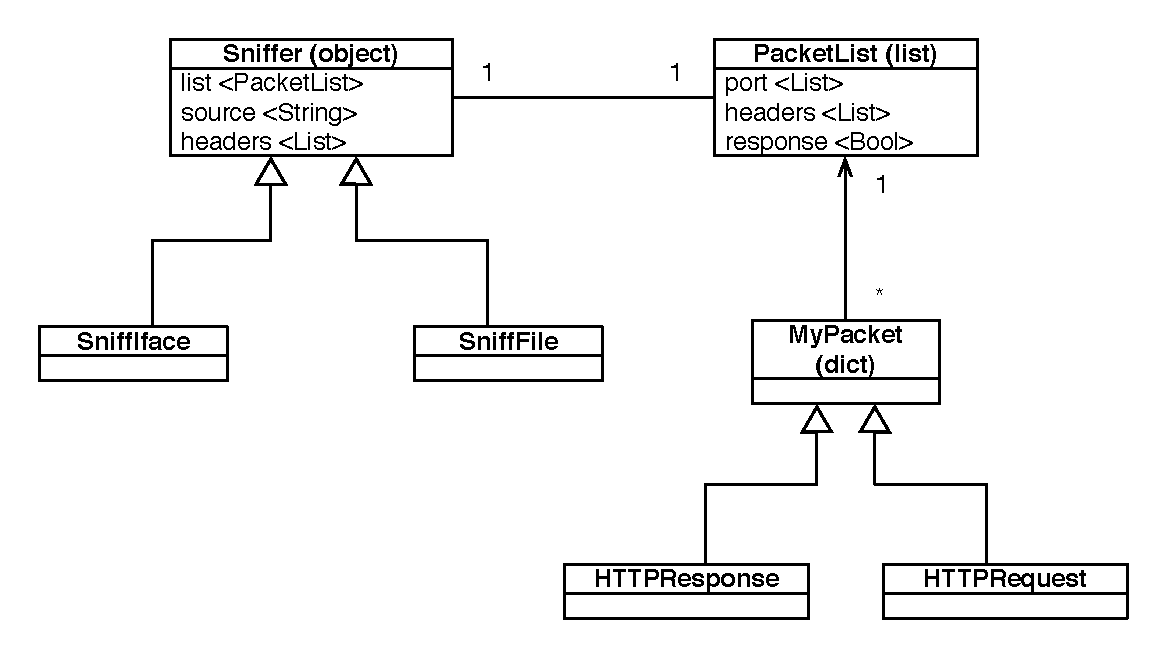
\includegraphics[width=0.65\textwidth]{./img/class.eps}
		\caption{Návrh tříd}
		\label{fig:label}
	\end{figure}

	% subsection navrh (end)

% section navrh_programu (end)


\section{Implementace} % (fold)
\label{sec:Implementace}

	\subsection{\texttt{HTTPpacket.py}} % (fold)
	\label{sub:HTTPpacket.py}
	V~uvedeném modulu je implementován seznam \texttt{PacketList}, u~kterého lze pomocí metody \texttt{append} vyvolat
	pokus o~přidání paketu (typ \texttt{Packet} definovaný knihovnou \texttt{scapy}) do tohoto seznamu. 
	Volání této metody spustí proces ověření, zda se v~paketu nachází HTTP požadavek nebo odpověď (definováno parametrem viz. \ref{sub:httphdrs}).
	V~případě kladného výsledku je do seznamu vložen objekt typu \texttt{HTTPRequest} nebo \texttt{HTTPResponse} odděděný
	od třídy \texttt{MyPacket}, která má za předka slovník. 

	\subsection{\texttt{utils.py}} % (fold)
	\label{sub:utils.py}
	Hlavním obsahem souboru je obecná třída \texttt{Sniffer}, která implementuje uložení paketů ze seznamu \texttt{PacketList}
	do výsledného XML souboru. Třída \texttt{Sniffer} je pak předkem třídám \texttt{SniffFile} a~\texttt{SniffIface}, ve kterých
	jsou implementovány metody pro získání vstupních dat. V~případě \texttt{SniffFile} se budou data načítat ze souboru 
	formátu \texttt{.pcap} a~ve druhém případě budou data odposlechnuty ze zadaného rozhraní (viz. \ref{sub:httphdrs}).

	\textit{Výsledný XML soubor} je generován vždy i~v~případě, že nedojde k~žádné shodě mezi získanými hlavičkami 
	ze vstupního zdroje a~hlavičkami specifikovanými parametrem případně výchozím seznamem. Minimální kostra je specifikována 
	zadáním. Jelikož není jasné, zda zadavatel nezamýšlí využívat výstupní data programu jako vstupní data jiného programu,
	tak výsledný soubor neobsahuje XML hlavičku (chybí v~příkladech výstupu aplikace i~její specifikaci).

	\subsection{\texttt{httphdrs.py}} % (fold)
	\label{sub:httphdrs}
	V~hlavním modulu programu jsou zpracovány parametry a~za zmínku stojí funkce \texttt{get\_input()}, která dle zadaných 
	parametrů vrátí objekt typu \texttt{SniffFile} nebo \texttt{SniffIface}, nicméně oba objekty mají stejného předka
	a~i~rozhraní, lze s~nimi tedy pracovat pomocí stejných metod (viz. funkce \texttt{main}). 

	\subsection{Použití} % (fold)
	\label{sub:pouziti}
	
\lstset{tabsize=2, breaklines, frame=single, basicstyle=\small}
\begin{lstlisting} 
ISA xpiste04$ python2.7 httphdrs.py -h
usage: httphdrs.py [-h] (-f FILE | -i IFACE) [-H HEADERS] [-p PORT] -o OUTPUT
                   [--extra]

arguments:
  -h, --help  show this help message and exit
  -f FILE     Pouzije jako vstup soubor ve formatu pcap.
  -i IFACE    Pouzije jako vstup rozhrani iface.
  -H HEADERS  Slouzi ke specifikaci sledovanych HTTP hlavicek. Case insensitive. 
  -p PORT     Slouzi ke specifikaci portu (muze jich byt vice).
  -o OUTPUT   Povinny parametr specifikuje nazev vyst. souboru.
  --extra     Rozsireni, ktere nebude ukladat HTTPRequest, ale HTTPResponse
\end{lstlisting}

	Při použití parametru \texttt{--extra} je funkcionalita ostatních parametrů zachována.
	Výchozí seznam hlaviček je pak změněn na \texttt{"Host,Location,Date,Status-Line,Server"}.

	\textit{Ukončení běhu programu} -- v~případně načítání hlaviček přes rozhraní stisk kláves
	\texttt{CTRL+C} ukončí odposlouchávání rozhraní a~provede zápis dat do XML souboru. V~jiných 
	případech, ale tato kombinace kláves program okamžitě ukončí!
	Přerušení běhu programu není nijak ošetřeno záměrně, protože program není cílen na běžné
	uživatele, ale na pokročilé uživatele, kteří pokud danou klávesovou kombinaci volí, 
	tak k~tomu mají důvod.

	% subsection pouziti (end)

	\subsection{Použité knihovny} % (fold)
	\label{sub:impl_knihovny}
	\begin{itemize}
		\item \texttt{Scapy} 	pro získání vstupních dat. 
		\item \texttt{Argparse} pro práci zpracování parametrů. 
		\item \texttt{Xml} 		pro výstup do XML souboru. 
		\item \texttt{Os} 		pro ověření možnosti práce se soubory. 
	\end{itemize}

	\subsection{Metriky kódu} % (fold)
	\label{sub:metriky_kodu}
	\begin{itemize}
		\item Počet řádků celkem: 341
		\item Počet řádků komentářů: 58
		\item Počet řádků zdojového kódu: 191
 	\end{itemize}

% section Implementace (end)

\section{Závěr} % (fold)
Výsledná aplikace by měla splňovat zadání v~plném rozsahu. Aplikace by mohla po rozšíření 
sloužit například pro jednoduchou firemní analýzu internetového provozu (hlavička \texttt{Host}
v~požadavcích klienta). 


\label{sec:zaver}

% section zaver (end)

\newpage

\bibliographystyle{csplainnat}
\renewcommand{\refname}{Literatura}
\bibliography{literatura}


\end{document}
